\label{chap:users_manual}

\section{About the FilmTit Application}

\emph{FilmTit} is a web application that assists amateur subtitle translators with translating movie and TV shows subtitles. In order to help save the amount of work spent on the translation, it provides suggestions on how the subtitles could be translated, based on a database of already existing translated subtitles.

You can translate any subtitle file you have from English to Czech or from Czech to English, making use of the millions of translations already made by other movie subtitles translators, coming from the tens of thousands of subtitle files in our database. From these, we always carefully select the most relevant ones for the lines that you are translating at the moment, which you can use as they are, post-edit them a little, or just use them for inspiration. And even if we find no similar lines in our database, there is always the machine translation system, ready to provide an automatically generated translation for any line you encounter.\footnote{Currently, the machine translation is only available for translation from English to Czech. Also please note that the machine translation can contain mistakes, as there is no perfect machine translation system in existence.}

Often it may be hard to fully understand the subtitles without seeing the movie; therefore, you have the possibility to load a movie file into the application, and the part of the movie that you are translating at a given moment will  always be played to you, also showing he source subtitles (and the target ones as well if you have already translated them). Most of the movie formats and codecs are supported!
% we dont have any other manual for the player than that paragraph I am afraid

FilmTit is a web application, which means you just have to open your favourite internet browser and you can start translating straight away -- no installation is necessary (although you may have to install Java and VLC for the video playback function, see Section~\ref{um:sec:installations}). However, this does not mean that you have to be online to translate the subtitles! Once you get all the translation suggestions from the server, you can go to the Offline Mode, work on the translation offline, and all your work will be automatically saved on the server when you are online again! See Section~\ref{um:sec:offlinemode}.

Similar to Google Documents, every single user operation is saved right after it is done -- there is no need for saving the documents manually; even if your browser crashes, you can continue working on the subtitle document exactly at the place where you ended last time.
%\todo{Note, Jo: But only if you have internet again? Well sure, there is the footnote saying that.}
Your data are available from any computer at any time exactly in the state you left them.\footnote{Except for the Offline Mode, where your data is saved to the server only when you go online again.}
\todo{The paragraph is more of an advertisement than truth. I would remove the whole para. We save the user translations transparently, yes. But this is the only place where this is done, everything else must be explicitely submited by the user. And even then, if he works in Offline Mode, he must then go online on the same computer in the same browser, so even then it is only half the truth.}

Similarly to Google Documents, you do not have to worry about saving your work -- your translations are automatically saved online right after you type them!
\todo{proposed new version of paragraph}

To run the application, you need a web browser with HTML5 support (Opera v.~12
Firefox v.~14, Chrome v.~21, Safari v.~5.1.5, or higher \todo{find versions exactly}). To use the optional video playback in your browser, you also need to have Java (at least version 1.6) and the VLC plugin (at least version 1.1.4).\todo{add it, who knows it -- I just added my versions, for which it works... RR}

\section{Installing Java and VLC Plugin}
\label{um:sec:installations}

Having installed Java and VLC Plugin is necessary for using the video playback in the application. It still of course possible to use the application without these plugins if you are not planning to use the video playback.

\subsection{Installing Java}

If you do not have Java installed, your browser will notice that automatically and will suggest you to install the missing plugin. If that happens, please follow the browser instructions.

If the installation via the browser fails, you will need to install Java manually, which is described in the following paragraphs.

\subsubsection{Windows}

For a manual installation, first download the Java Installer from the \emph{java.com} website. Go to \url{http://www.java.com} and click on ``Free Java Download'' button. The website will propose a suitable version for you. (If you want to download a different version, click on the ``See all Java downloads'' link.) It is recommended to check the system requirements of the version you are going to download and to read the license conditions.

After launching the installation guide, simply follow the instructions displayed. For a more detailed description of the installation, please see \url{http://www.java.com/en/download/help/windows_manual_download.xml}.

After finishing the installation, it is necessary to restart your browser.
(It is recommended to reboot the whole system.)

\subsubsection{Linux}

To install Java on a Linux system, download the installation package similarly as is described for Windows. To do the installation from the command line, please follow the instructions at \url{http://www.java.com/en/download/help/linux_install.xml#install}. (It might not be enough to just install Java -- it may also be necessary to manually enable Java in your browser. The instructions can be found on the same website.)

After finishing the installation, it is necessary to restart your browser.

\subsection{Installing VLC Plugin}

The VLC player plugin is available only for Firefox, Chrome, Opera and Safari. Internet Explorer uses an \emph{ActiveX} VLC plugin which is not supported by our application; therefore, video playback unfortunately does not work in Internet Explorer.

If you already have an installation of the VLC player without the plugin, it is necessary to reinstall the whole VLC player. It is not necessary to uninstall it manually, it is done automatically with the new installation.

To install the VLC player with the plugin on Windows, download the installation program from \url{http://www.videolan.org/vlc/}. The web page should suggest you a suitable version for your computer. If you want to install a different version, click on ``Other Systems and Versions'', otherwise just click the ``Download VLC'' button.

\begin{figure}[h]
\begin{center}
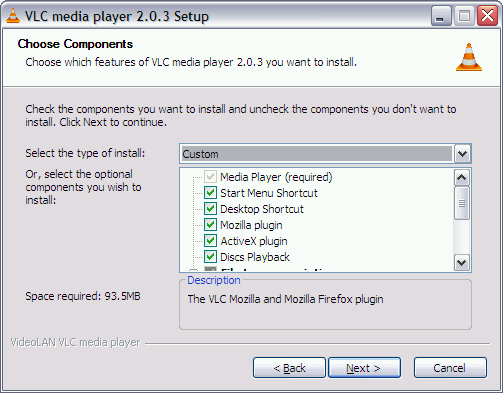
\includegraphics[scale=0.4]{figures/vlc_installation.png}
\end{center}
\caption{Installation guide of VLC player for Windows.}
\label{fig:vlc}
\end{figure}

To install the plugin, do not forget to tick the box with ``Mozilla plugin'' label in the third step of the installation guide (named Choose Components, see Figure~\ref{fig:vlc}). After finishing the installation, it is necessary to restart your browser.

Instructions for installation on Linux systems can be found at \url{http://www.videolan.org/doc/vlc-user-guide/en/ch03.html}


\section{Registration and Login}
\label{um:sec:login}

We require the users to be logged into the application during their work. We do so to enable the users to save their work and return to it another time. However, there is also an Offline Mode, where the data is stored locally in your computer and uploaded to server once you go online -- see Section~\ref{um:sec:offlinemode}.

\subsection{Registration and Basic Login}

The first option how to get an account to the application is to register and get a user name and password, similarly to any other web application. However, if you have a Google, Yahoo or Seznam account, we recommend you to use the ``OpenID login'', which enables you to use your already existing account at Google, Yahoo or Seznam to log into the FilmTit application.

\begin{figure}[h]
\begin{center}
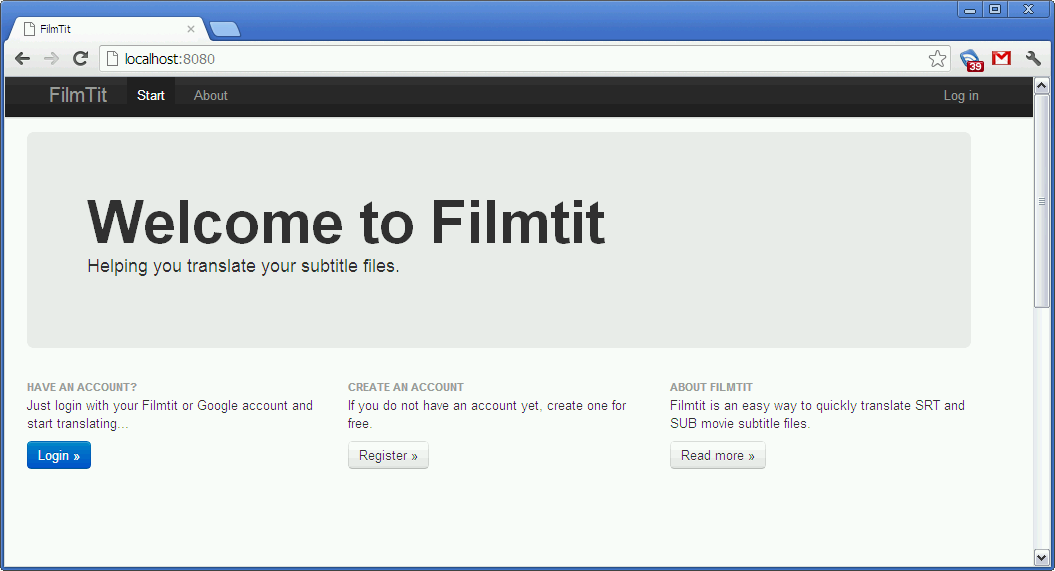
\includegraphics[scale=0.4]{figures/user_manual/welcome_screen.png}
\end{center}
\caption{Welcome screen of the application.}
\label{fig:welcome}
\end{figure}

For the classic registration, click the ``Register'' button on the Welcome screen (Figure~\ref{fig:welcome}) or click the ``Login'' button and select the third tab in the opened dialog (Figure~\ref{fig:register_login}).

After that, you are requested to choose a user name, fill in a valid a email address and type twice the password you would like to use. (You do not need to fill in an email address, but it is necessary for password recovery in case you forget your password.) Because the application does not contain any sensitive information, we try to keep the registration and login process as simple as possible and there are no requirements on the strength of the password (except for a minimum length of 3 characters). After a successful registration, you will receive an email confirming the registration.

\begin{figure}[h]
\begin{center}
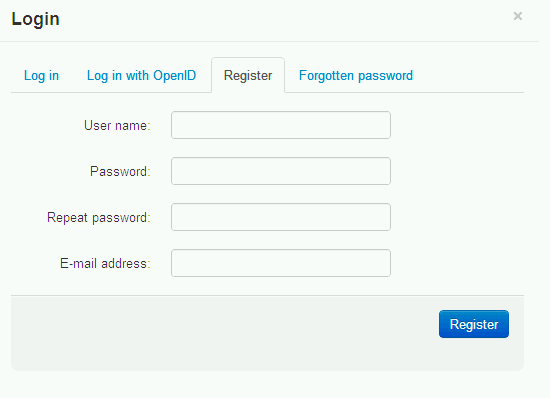
\includegraphics[scale=0.4]{figures/user_manual/register.png}~~~~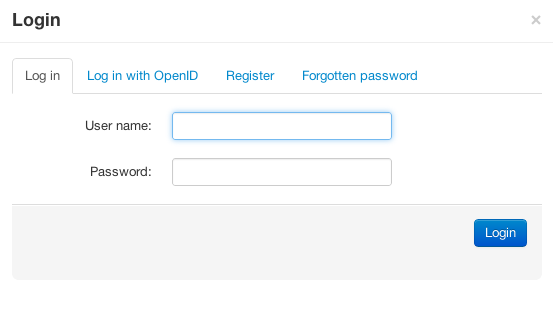
\includegraphics[scale=0.4]{figures/user_manual/login.png}
\end{center}
\caption{Registration form and login form.}
\label{fig:register_login}
\end{figure}

You are automatically logged in after the registration. For logging in next time, click on the login button on the welcome screen and fill in your user name and password (Figure~\ref{fig:register_login}). Your login session is valid for 1 hour -- if you do not use the application for 1 hour, you will be logged out automatically. If you want to stay logged in permanently, you can set this in the settings, see Section~\ref{sec:settings}.

\subsection{OpenID Login}

Another option to log into the application is using Google, Yahoo or Seznam account. After choosing the service you want to use, a pop-up window is opened. It may happen that your browser blocks this window -- if this happens, you need to allow the pop-up window to continue the logging process.

You will see the login form of the service you have chosen. If you are currently already logged into the service, you will only see the confirmation request to allow the FilmTit application to access your account data (it is your user name in the service, your first name, surname, email and gender, depending on what you filled in in the particular service and what you allowed to be provided to the third party applications, but it is never the password to the original service). \todo{why do we get the name and gender if we dont use it??? RR}
After submitting your user name and user password and confirming that the FilmTit application can receive your authentication data, the pop-up window will be automatically closed. Within a few seconds you will be redirected to the list of documents you own (if this is your first time logging into the application, you have no documents yet, so you will see the New Document page instead).

If you use OpenID Login, you do not have to register -- you are registered automatically on your first successful login. You also automatically get a user name and password for the Basic Login, which is sent to your e-mail address upon registration (if your OpenID provider provides us with one) and can be changed in the Settings.

\subsection{Forgotten Password}

Another issue connected to login is dealing with the situation when users forget their passwords. If such a situation happens, open the login dialog and click on the "Forgotten password" tab. Fill in either your user name or email (or both) and click "Send password change link to email" (see Figure~\ref{forgotten_pass}). (Please note that if you did not set a valid e-mail address with your account, you cannot use this feature.)

\begin{figure}[h]
\begin{center}
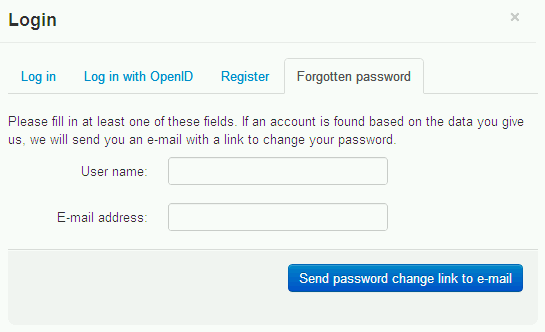
\includegraphics[scale=0.4]{figures/user_manual/forgotten_password.png}
\end{center}
\caption{Form for requesting the forgotten password.}
\label{fig:forgotten_pass}
\end{figure}

After that, you will receive an email containing your user name with a link to a page where you can change your password. If you ignore the email, the original password will remain valid.

\section{Changing the User's Settings}
\label{sec:settings}

You can change the user settings by clicking the Settings link in the top menu of the application (you must be logged in to have the Settings available). You can see the settings form in Figure~\ref{fig:settings}. After you are done with changing the settings, click the Save button.

\begin{figure}[h]
\begin{center}
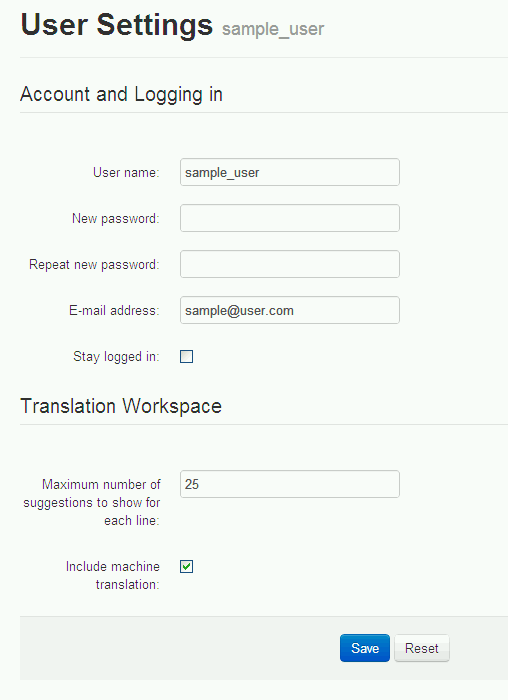
\includegraphics[scale=0.4]{figures/user_manual/user_settings.png}
\end{center}
\caption{The settings form}
\end{figure}

\subsection{Account and Logging in}
\subsubsection{User name}

The user name has to be unique in the FilmTit application. If users use the classic registration form, they can choose their own user name. If a user wants to register a user name which already exists, the application displays warning. Registration by openID is the second way how to receive a user name. The user name from this registration is extracted from the email address.
There is a chance that two users have a very similar email address and the extracted name will be the same. Our app generates the user name with a unique numeric code in this case. 
The user name can be changed in the page User Settings.


\subsubsection{New password}

You can change your password by filling the two boxes with two identical strings which will become your new password. As was already mentioned, we do not have any requirements on the strength of the password except for a minimal length of 3 characters.

By leaving the two input boxes empty, the old password remains unchanged.

\subsubsection{E-mail address}

In this input box, you can change you email address. It is checked whether the address has a valid email address format, but we do not test the email address' existence and functionality. We recommend to fill in a working email address for the case that you forget your password.

\subsubsection{Stay logged in}

By ticking this option you stay permanently logged in to the application -- unless you log out. (After a really long time of not appearing in the application, you will be automatically logged out for security reasons; it is a month by default, but it depends on the administration settings of the server.)

\subsection{Translation Workspace}

There are also some options concerning the translation workspace. To fully understand the options, please read Section~\ref{sec:document_editing} first.

\subsubsection{Maximum number of suggestions to show for each line}

It is the maximum number of suggestion that can be displayed for a particular subtitle chunk being translated. It can be any number between 1 and 100. To work efficiently with the translation suggestion, we recommend to use at most 25 suggestions.

\subsubsection{Include machine translation}

By this option you indicate if you want to include automatic translation among the translation results. If this option is disabled, you receive only sentences which have occurred before in the subtitle files that we have available in our database.

The machine translation provides automatically generated sentences by the open-source statistical machine translation system Moses. When we tested it on the subtitle data, it performed better than the popular Google Translate system (tested in August 2012).

If you disable the machine translation, you often do not receive any suggestions for chunks. However, you get the suggestions faster (the machine translation is usually the slowest part of the suggestions generation process), and all suggestions you get are human translations which generally have a higher quality than the automatic translations.

Please note that in the current version, machine translation is only available for translations from English to Czech.

\section{Creating a New Document}
\label{um:sec:doccreation}

A document is a subtitle file in the source language (usually English) which you load into the application, together with its translation in the target language (usually Czech) which you produce with the help of the application. Creating a document means loading a subtitle file in the source language and starting to translate it. You can create a new document either by clicking the ``Create a new document'' button in the document list, or by clicking the ``New document'' link in the top menu.

\begin{figure}[h]
\begin{center}
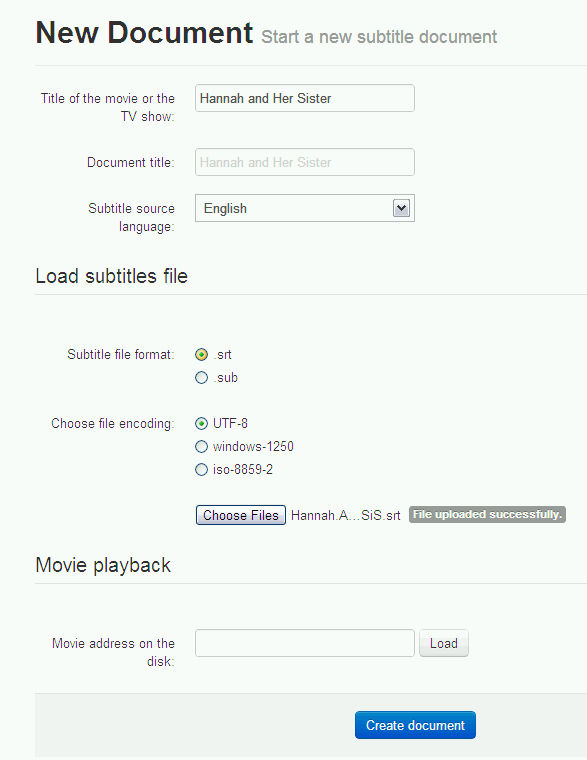
\includegraphics[scale=0.4]{figures/user_manual/new_document.png}
\end{center}
\caption{Form for creating a new document.}
\end{figure}

While creating a document, you are asked to fill in the movie title and the document title (which defaults to the movie title, but you can set any name you like). In the case of TV series, please fill in the name of the series, not the name of the particular episode. An example of it can be to type ``Lost'' as the movie title and ``Lost S01E01'' as the document title. Then you are asked to choose the source language of the subtitles, encoding of the subtitle file and the path to the actual subtitle file you would like to translate. You should also make sure you selected the proper encoding of the source subtitle file. You can choose from UTF-8, windows-1280 and iso-8859-2, which are the most commonly used encodings for Central European languages. (Usually UTF-8 is the correct choice.)

There is also an option to play the video of the movie you have on your computer. If you want to do so, click the "Load" button below the "Movie playback" headline and select the movie file. For this step you need to have Java and the VLC plugin installed as was mentioned before. Please be patient while doing it, loading the open file dialog can take a while on slower computers. 
%(The browsers do not normally support opening the local files without posting them to the server, therefore we had to develop a non-standard solution.) \todo{the last sentence does not bother I user I am afraid, I would delete it}

Then you can submit the document. Within seconds, a form containing movies with the title you provided should appear (see Figure~\ref{fig:media_sources}).

\begin{figure}[h]
\begin{center}
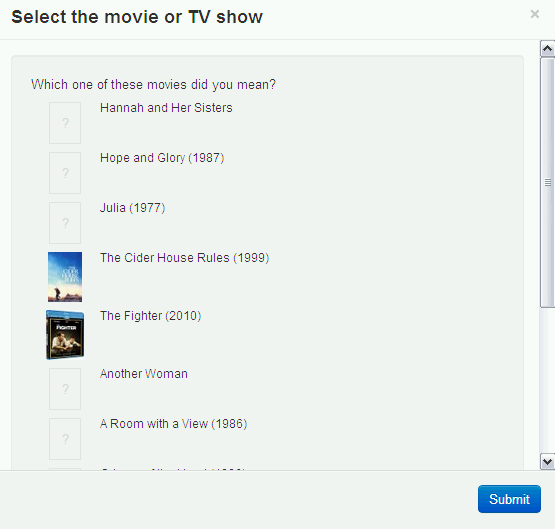
\includegraphics[scale=0.4]{figures/user_manual/media_sources.png}
\end{center}
\caption{Form for selection of a movie. It shows the suggestion after a misspelled title of Woody Alan's movie "Hannah and Her Sisters" was submitted.}
\label{fig:media_sources}
\end{figure}

After clicking on the movie you meant, click submit and you can start editing your new document. In case you do not like the suggested movies at all, you can click the cross in the top right corner of the form and try to reset the movie later in the document list.

\section{Document Editing}
\label{sec:document_editing}

When you start editing a document, either a new one or an existing one, you see the translation workspace, see Figure~\ref{fig:translation_workspace}. It has three columns. In the first column, there are the timings of the subtitles, in the middle column you can see the subtitles in the original language and in the third column there are the text boxes ready to be filled in by the translation in the target language.

Immediately after you open the translation workspace the translation suggestions starts to be loaded.

\begin{figure}[h]
\begin{center}
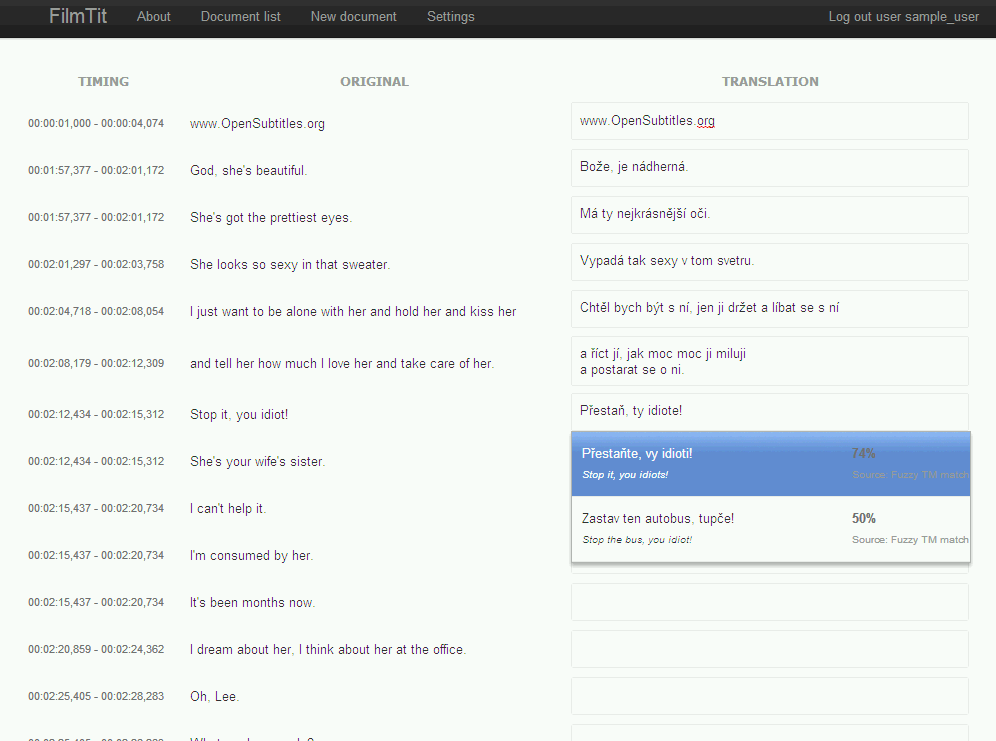
\includegraphics[scale=0.4]{figures/user_manual/translation_workspace.png}
\end{center}
\caption{The translation workspace during translating a document.}
\label{fig:translation_workspace}
\end{figure}

After the translation suggestions arrive to the translation workspace, you can write down your translations.  (You can edit it even if the suggestion does not arrive, but will not be able to see the suggestions.) The translation suggestions appear below the text area where the text cursor is in. You can select one of the suggestions by clicking on them or using the arrow keys and post edit it then. You can also write the translation from scratch and ignore the suggestion. You can add a line break by pressing \emph{Enter}.

To move to the next subtitle chunk just click to the next text box or press the \emph{Tab} key. If you want to move to the previous subtitle chunk, press \emph{Shift + Tab}.

You can change the subtitle timing by double-clicking on it or the text of the original subtitle also by double-clicking on it. If you change the text for the particular subtitle, the suggestions are regenerated. It may take some time to the new suggestions to appear.

It is not necessary to save your work in any way, everything is save right after it is edited, so you can leave the document by clicking on a link or even close the browser and nothing will be lost. If the Internet connection breaks down you can continue working on the in the Offline Mode which is described in the following section.

\section{Offline Mode}
\label{um:sec:offlinemode}

When the application realizes that it cannot connect to the server, it offers you to continue in Offline Mode (see Figure~\ref{fig:start_offline_mode}). When you turn on the Offline Mode, you can continue translating the document -- all translation suggestions that have already been loaded will be shown to you and all translations that you enter will be saved.
(However, you cannot list the documents, open or create another document, or export or delete the documents.)

%\todo{you also cannot change the timing or the source text, although this would be perfectly possible: however, I have not added support for that, which I might probably do now}
% not adding support for that since nobody seems to care

If you refuse starting the Offline Mode, all the editing done without the Internet connection will be lost!

\begin{figure}[h]
\begin{center}
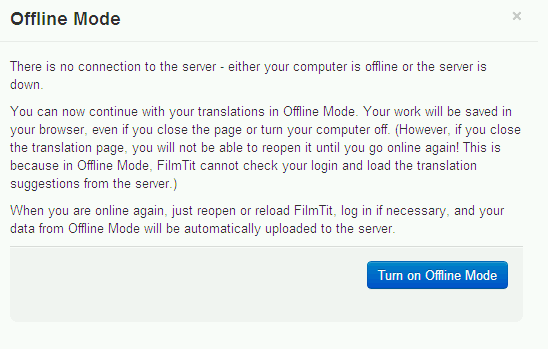
\includegraphics[scale=0.4]{figures/user_manual/offline_mode.png}
\end{center}
\caption{Confirmation request for start the offline mode.}
\label{fig:start_offline_mode}
\end{figure}

During the work in Offline Mode, all the operations are stored in the browser. Once you leave the page with the translation workspace, you cannot continue editing the file -- however, you can even close your browser or restart the computer, and still all the changes that you have made on the document in Offline Mode will be saved.

The data from the Offline Mode are posted to the server at the time you log in to the application the next time after you confirm you want to do so (see Figure~\ref{fig:offline_loading}). If your Internet connection starts to work during your work in Offline Mode, you can just reload the page in your browser, log in and continue with your work.

The information in Offline Mode are bound to your computer, browser and user. So, to be able to upload the Offline changes to the server, you have to log in on the same computer as the same user and use the same browser.

\begin{figure}[h]
\begin{center}
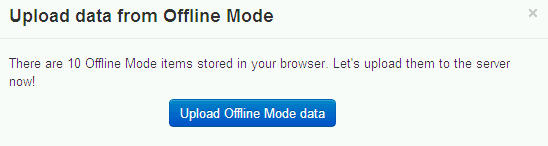
\includegraphics[scale=0.4]{figures/user_manual/upload_offline_mode.png}~~~~
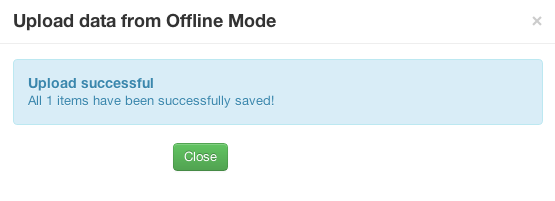
\includegraphics[scale=0.4]{figures/user_manual/upload_offline_mode_success.png}
\end{center}
\caption{Loading data from the Offline Mode}
\label{fig:offline_loading}
\end{figure}

\section{Operations with Documents}
\label{um:sec:docoperations}

You can list your documents by clicking on the "Document list" link in the top navigation of the application, see Figure~\ref{fig:document_list}. You can edit the document by clicking on the "Edit" button.

\begin{figure}[h]
\begin{center}
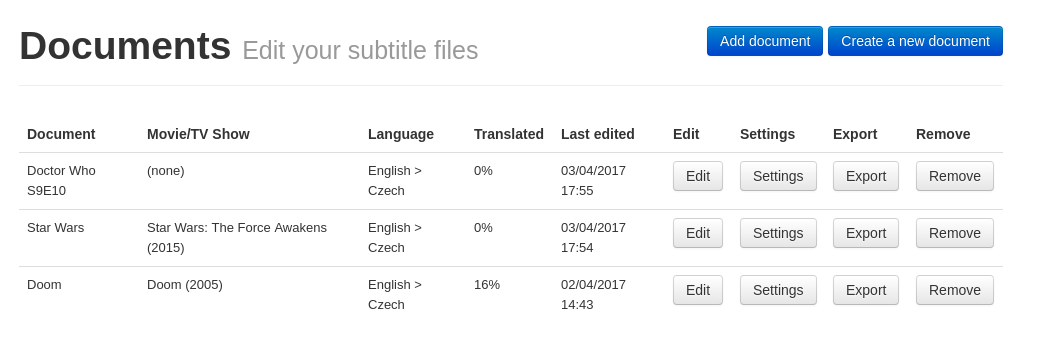
\includegraphics[scale=0.4]{figures/user_manual/list_of_documents.png}
\end{center}
\caption{List of documents owned by the user}
\label{fig:document_list}
\end{figure}

Clicking on the export button will open a dialog for downloading the subtitle file based on the document. You can select if you want to download the subtitles in the source language, the translated version or the translated version with the original subtitles where the document remained untranslated. After clicking on a button with the required format, the download of the subtitle file will start.

By clicking the delete button you will remove the document from you document list.

You can also change the title of the document, by clicking on the title and typing the original or change the movie title. If change change the name of movie, the same dialog as while creating a document will show (Figure~\ref{fig:media_sources}) where you can select the movie you meant.
